%% ------------------------------------------------------------------------- %%
\chapter{Resultados Preliminares}
\label{cap:resultados}
	A partir dos algoritmos estudados, escolhemos dois algoritmos para passarem em três testes para determinar sua 
eficâcia. O primeiro escolhido foi o \textit{Demons}, dada a facilidade em adotar a arquitetura SIMD, sua popularidade 
dentro da área de processamento de imagens médicas e seu poder em registrar pequenas deformações com baixo custo 
computacional. O outro escolhido foi o TPS, que com seu método de registro que utiliza características, permite que ele
seja aplicado a uma gama maior de tipo de imagens e os vários pontos em que ele pode ser acelerado. Os testes pelos 
quais os algoritmos passaram estão descritos abaixo.

%% ------------------------------------------------------------------------- %%
%% ------------------------------------------------------------------------- %%
\section{Testes}
	Os testes foram inspirados pelo estudo de \cite{zagorchev2006comparative}. Foram escolhidos três tipos
de deformações para validar a eficácia dos algoritmos apresentados acima. A imagem Referência utilizada para os
testes foi retirada do software BioImage \cite{papademetris2005bioimage}. Todas as imagens Alvo são resultados
das deformações escolhidas aplicadas a imagem Referência.

	A primeira deformação aplica uma distorção senoidal nos dois eixos da imagem Referência, com a
seguinte equação:
\begin{align} \label{math:sin}
\begin{split}
	X &= x - 8sin(x/32) \\
	Y &= y + 4cos(x/16)
\end{split}  	
\end{align}
	Esse teste tem como finalidade determinar a eficácia dos algoritmos em registrar imagens que sofreram
ação de uma deformação global, ou seja, ela é totalmente uniforme sob toda a imagem.

	A próxima deformação utiliza a distância do pixel até o centro da imagem para determina. A deformação
é definida por:
\begin{align} \label{math:dist}
\begin{split}
	X &= x + 50(x-x_m)/r \\
	Y &= y + 50(y-y_m)/r 
\end{split} 
\end{align}

Onde $x_m$ e $y_m$ são o número de linhas e colunas, respectivamente, divididos por 2 e $r = \sqrt{(x-x_m)^2 + (y-y_m)^2}$
define uma circunferrência centrada no centro da imagem. Essa deformação testa a capacidade dos algoritmos de registrar
deformações locais, que agem de maneira não uniforme em toda a imagem.

	A última deformação é uma combinação das duas já apresentadas:
\begin{align} \label{math:composta}
\begin{split}
	X &= x-8sin(y/16) + 50(x-x_m)/r \\
	Y &= y+4cos(x/32) + 50(y-y_m)/r
\end{split} 
\end{align}
	Ela testa tanto a capacidade de registrar deformações complexas, que tem tanto uma fração global quanto uma local. 
Exemplos das três deformações estão na figura \ref{fig:deformacoes}.

\begin{figure}[H]
    \centering
	\begin{subfigure}[t]{0.3\textwidth}
	  
\includegraphics[width=\textwidth]{figuras/grid.png}
	  \subcaption*{(a)}
	  \label{fig:ref-image}
	\end{subfigure}
	\begin{subfigure}[t]{0.3\textwidth}
	  
\includegraphics[width=\textwidth]{figuras/gridSin.png}
	  \subcaption*{(b)}
	  \label{fig:ref-image}
	\end{subfigure} \\
	\begin{subfigure}[t]{0.3\textwidth}
	  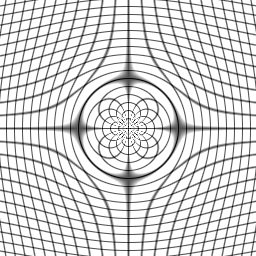
\includegraphics[width=\textwidth]{figuras/gridDist.png}
	  \subcaption*{(c)}
	  \label{fig:sin-image}
	\end{subfigure}
	\begin{subfigure}[t]{0.3\textwidth}
	  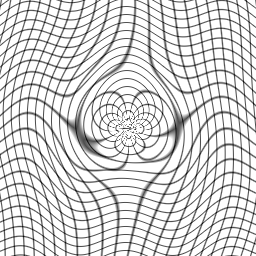
\includegraphics[width=\textwidth]{figuras/movingImageDistSin.png}
	  \subcaption*{(d)}
	  \label{fig:dist-image}
	\end{subfigure}
	\caption{Grade (a) deformada por: (b) deformação seno \ref{math:sin}; (c) deformação por distância \ref{math:dist}; 
				(d) deformação composta \ref{math:composta}. }
	\label{fig:deformacoes}
\end{figure}

	As imagens criadas pelos métodos descritos já são o suficiente para os testes com o \textit{Demons}, mas o TPS
necessita de características e de suas correspondências. As características necessárias para a execução do TPS foram 
criadas utilizando uma grade oito por oito de pontos uniformemente distribuidos para a imagem Referência. As suas 
correspondentes nas imagens alvo foram calculadas aplicando as deformações adequadas as caracteristicas da imagem 
Referência.

%% ------------------------------------------------------------------------- %%
%% ------------------------------------------------------------------------- %%
\section{Avaliação dos testes}

\begin{figure}[h]
	\centering
	\begin{subfigure}[t]{0.23\textwidth}
	  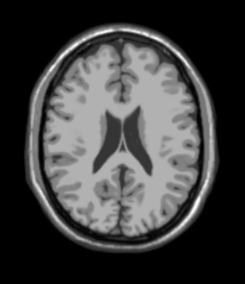
\includegraphics[width=\textwidth]{figuras/screen.png}
	  \subcaption*{(a)}
	  \label{fig:ref-image}
	\end{subfigure}
	\begin{subfigure}[t]{0.23\textwidth}
	  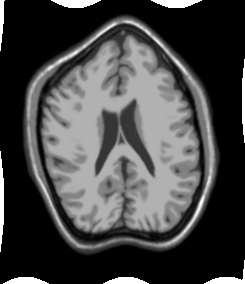
\includegraphics[width=\textwidth]{figuras/movingImageSin.png}
	  \subcaption*{(b)}
	  \label{fig:sin-image}
	\end{subfigure}
	\begin{subfigure}[t]{0.23\textwidth}
	  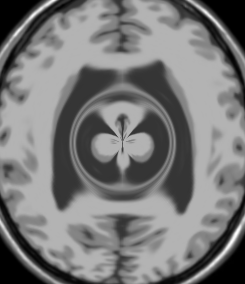
\includegraphics[width=\textwidth]{figuras/movingImageDist.png}
	  \subcaption*{(c)}
	  \label{fig:dist-image}
	\end{subfigure}
	\begin{subfigure}[t]{0.23\textwidth}
	  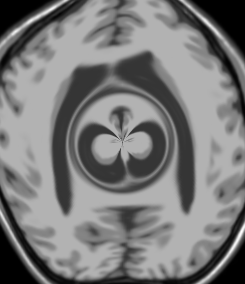
\includegraphics[width=\textwidth]{figuras/movingImageSinDist.png}
	  \subcaption*{(d)}
	  \label{fig:sindist-image} 
	\end{subfigure} \\
	\begin{subfigure}[t]{0.25\textwidth}
	  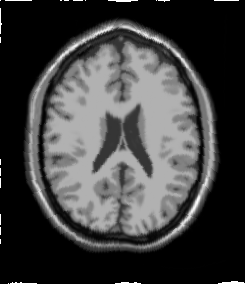
\includegraphics[width=\textwidth]{figuras/resultSin.png}
	  \subcaption*{(e)}
	  \label{fig:sin-image-tps} 
	\end{subfigure}
	\begin{subfigure}[t]{0.25\textwidth}
	  
\includegraphics[width=\textwidth]{figuras/resultDist.png}
	  \subcaption*{(f)}
	  \label{fig:dist-image-tps}
	\end{subfigure}
	\begin{subfigure}[t]{0.25\textwidth}
	  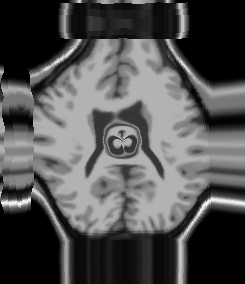
\includegraphics[width=\textwidth]{figuras/resultDistSin.png}
	  \subcaption*{(g)}
	  \label{fig:sindist-image-tps} 
	\end{subfigure} \\
	\begin{subfigure}[t]{0.25\textwidth}
	  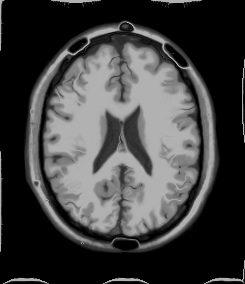
\includegraphics[width=\textwidth]{figuras/resultSinDemon.png}
	  \subcaption*{(h)}
	  \label{fig:sin-image-demon}
	\end{subfigure}
	\begin{subfigure}[t]{0.25\textwidth}
	  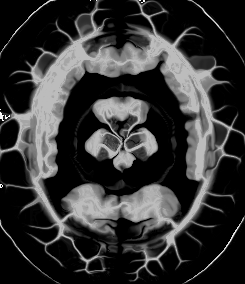
\includegraphics[width=\textwidth]{figuras/resultDistDemons.png}
	  \subcaption*{(i)}
	  \label{fig:dist-image-demon}
	\end{subfigure}
	\begin{subfigure}[t]{0.25\textwidth}
	  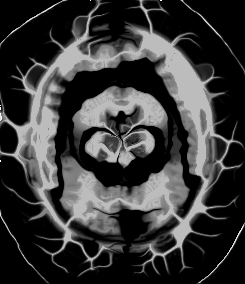
\includegraphics[width=\textwidth]{figuras/resultSinDistDemon.png}
	  \subcaption*{(j)}
	  \label{fig:sindist-image-demon}
	\end{subfigure}
	\caption{(a) imagem Referência. (b) imagem Alvo deformada pela função seno. (c) imagem Alvo deformada pela função 
			distância. (d) imagem Alvo deformada pela função composta. (e) imagem Registrada entre (a) e (b) pelo TPS. 
			(f) imagem Registrada entre (a) e (c) pelo TPS. (g) imagem Registrada entre (a) e (d) pelo TPS. (h) imagem 
			Registrada entre (a) e (b) pelo Demons. (i) imagem Registrada entre (a) e (c) pelo Demons. (j) imagem 
			Registrada entre (a) e (d) pelo Demons.}
	\label{fig:resultados}
\end{figure}
	Os resultados dos testes podem ser observados na figura \ref{fig:resultados}.
Os dois algoritmos tiveram um resultado satisfatório registrando o primeiro teste, enquanto somente um deles conseguiu
registra os dois últimos testes com um resultado aceitável, dada a natureza não uniforme da distorção utilizada. 
No primeiro teste, com a deformação sinoidal \ref{math:sin}, o resultado obtido pelos dois algoritmos foi satisfatório.
A diferença entre os métodos de registro são claramente vistos observando as imagens resultado de cada método. Podemos
notar a maior suavidade da imagem gerada pelo \textit{Demons} em comparação ao registro pelo TPS, pela utilização do
filtro Gaussiano do \textit{Demons}. O TPS foi capaz de manter a estrutura anatômica do cerebro, enquanto o 
\textit{Demons} não foi capaz de tal feito dada a natureza difeomorfica do seu algoritmo. Por final, nenhum dos 
algoritmos conseguiu registrarb com eficácia a borda, já que a deformação faz com que alguns pixels caiam fora da 
imagem, mas isso é esperado.

  Já no segundo e no terceiro teste, a deformação aplicada ao centro foi muito intensa, logo era esperado a baixa 
eficácia dos algoritmos nessa região. O TPS se mostrou melhor ao \textit{Demons} nas regiões entorno do centro, 
conseguindo registrar a imagem com algum sucesso. A medida que a força da distorção diminui, os resultados do TPS 
melhoram. As bordas da imagem ficaram com uma qualidade ruim dado o método de geração das características. Quando a 
grade uniforme de características passa pela deformação, várias característcas ficam aglomeradas nas bordas da imagem, 
o que compromete o resultado nesse caso.

	Já o \textit{Demons} obteve um resultado com uma qualidade inferior pois a fórmula usada para cálcular o campo 
vetorial \ref{math:demons} utiliza o gradiente das duas imagens para calcular a direção da transformação do registro. 
Como a distorção usada nesse teste foi caótica, a transformação obtida fez com que pontos próximos fossem mapeados para 
pontos distantes na imagem Referência, levando ao resultado obtido.